\index{Observing!Test Steps}
\index{Test Step!Observe}
\label{TasksObserveJava}

\bxtipp{If you have not already done so, we recommend reading the tips section for the observation mode before beginning observing \bxpref{TasksObsModeTips}. }
\begin{enumerate}
\item  In Java \gdauts{} (Swing and SWT/RCP, but not GEF components in RCP) the observation mode will automatically record your actions in the user interface. Each action is created as a \gdstep{} in the \gdtestcaseeditor{} for this observed \gdcase{}. 

\bxtipp{See the section later on performing check actions in the observation mode \bxpref{TasksObsCheckJava}.}

\item You can also see which actions have been recorded in the console (\bxfigref{obsconsole}).

\begin{figure}[h]
\begin{center}
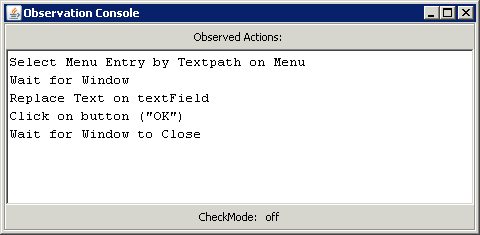
\includegraphics{Tasks/Recording/PS/obsconsole}
\caption{The observation console}
\label{obsconsole}
\end{center}
\end{figure}


\bxtipp{If you are creating tests for SWT and RCP \gdauts{}, check that you have set the keyboard layout correctly in the \gdproject{} properties \bxpref{AdvancedAUTConfig} and that you have defined the right toolkit for the \gdproject{} \bxpref{ProjPropertiesChangingToolkit}.}
 

\item Component names for your components are automatically generated and assigned to the technical names from the \gdaut{} when you observe \gdsteps{}. If you have already created and mapped a component name for a technical component, this name will be used instead of creating a new one. 
\item Once you have recorded the actions you need, stop the observation mode by clicking on the \bxcaption{stop observing \gdcase{}} button 
\gdmarpar{../../../share/PS/stopcam}{stop observation}
on the main toolbar.
\item Save the \gdcase{} editor containing the \gdsteps{} you have just observed. 
\item Check the \gdsteps{} and their parameter values which have been recorded. 
You will notice that any text that contains non-alphanumeric characters is enclosed in single quotes. Single quotes are used  to cancel any meaning of the characters within the quotes. 
\bxtipp{Run the test that you have just recorded to see if it works as you intended. If not, you may need to make some changes to the parameter values, or you may have to supplement the \gdcase{} with \gdcases{} from the library \bxpref{UseLibrary}. }
\end{enumerate}

\subsubsection{Actions that cannot be recorded}
A few actions cannot be recorded in the current version. These include:
\begin{itemize}
\item Key combinations that are used as shortcuts in SWT applications.
\item Click counts on trees. The select actions are correctly recorded, but the click count is set to 0 and must be manually adjusted. 
\item Components that contain texts that are too long (more than 3999 characters). 
\item Actions on native dialogs e.g. file choosers. 
\item Actions in the figure canvas for GEF components. 
\end{itemize}

\subsubsection{Performing checks in the Java observation mode}
\label{TasksObsCheckJava}

You can perform checks in the observation mode by taking the following steps:
\begin{enumerate}
\item Start the check mode by pressing \bxkey{Ctrl+Shift+F11}. This key combination can be changed in the preferences \bxpref{TasksPrefsObsModeJava}. 
\item In the observation console, the check mode will be marked as \bxname{on}. 
\item In the \gdaut{}, components will be highlighted with a red border (\bxfigref{redborders}).

\begin{figure}[h]
\begin{center}
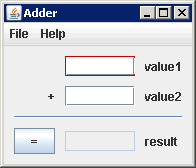
\includegraphics{Tasks/Recording/PS/redborders}
\caption{Red borders in the check  mode}
\label{redborders}
\end{center}
\end{figure}
 
\bxtipp{While the check mode is active, no other actions will be recorded.}
\item Hover over the component you want to execute a check on and press \bxkey{Ctrl+Shift+F12}. This key combination can be changed in the preferences \bxpref{TasksPrefsObsModeJava}. 
\item A dialog will appear showing the type of component you are performing the check on. 
\item From the dialog, select the check action you want to perform and enter any parameters the check action needs. Many check actions have predefined parameters based on the state of the \gdaut{}. 
\item When you have specified your check action, choose whether you want to close the dialog and continue in the check mode (\bxname{check on}) or whether you want to stop the check mode when the dialog closes (\bxname{stop checking}). 
\bxtipp{You can manually stop the check mode using the same key combination as you used to start the check mode (\bxkey{Ctrl+Shift+F11} by default).}
\item The check action you specify will be added to the \gdtestcaseeditor{}. 
\end{enumerate}




  


